\documentclass[a4paper]{article}

\usepackage[english]{babel}
\usepackage[utf8x]{inputenc}
\usepackage{amsmath}
\usepackage{graphicx}
\usepackage[colorinlistoftodos]{todonotes}
\usepackage{parskip}
\usepackage{float}
\usepackage{hyperref}
\usepackage{fullpage}
\usepackage{listings}
\usepackage[T1]{fontenc}

\lstset{
	numberstyle=\footnotesize,
	basicstyle=\footnotesize\ttfamily,
	breaklines=true
}

\begin{document}

\title{Assignment 1 \\ Secure Data Management}
\author{Rick van Galen - s0167746 (UT) \\ Erwin Middelesch - s0197106 (UT) \\ Jeroen Senden - s0191213 (UT) \\ Bas Stottelaar - s0199141 (UT)}
\date{\today}
\maketitle

\section{Introduction}
	In this report, we describe our prototype implementation for a Public Health Record (PHR) system. This system is implemented in Python and consists of a client and server. The role of the server is to announce the public parameters and store encrypted data while the client takes care of the encryption and decryption of data.

	Our solution is based on a Ciphertext-Policy Attribute-Based Encryption (CP-ABE) scheme and uses no classic access control to authenticate users. Different categories of data can be read and written by different parties or sub parties.
	
	First, we introduce the data model, including the categories of data and different parties. Then, we introduce the access policies. The third section will discuss the actual implementation and verifies the the requirements. The last section will discuss our implementation.

\section{Data model}
	This section defines the categories of data and the parties involved.

	\subsection{Data categories}
		The system defines the categories below. 
		
		\begin{description}
		    \item[Patient data]
		    In this segment of the health record, we store personal information of the user. 
		    \item[Health data]
		    This is the data inserted by a hospital where the user has been treated.
		    \item[Training data]
		    This section contains training related data stored by the health club.
		\end{description}
		
	\subsection{Parties}
		The following parties are defined and assumed to work with the system. For this prototype, we consider them to be honest.
		
		\begin{description}
			\item[Patient] The subject of the electronic health system. Each health record is associated with one patient and should be under full control of the patient. The patient has full read and write access to every category of data.
			\item[Doctor] A patient's doctor treats the patient with health issues. The doctor may require read access to any part of a patient's health record. Therefore, the patient may choose to give the doctor read access to his personal information, health data and training data.
			\item[Insurance] Health insurance companies may want to read a patient's records for fee calculations or health verification. A patient may give insurance companies read access to (a part of) his record.
			\item[Employer] Like the insurance company, an employer may need access to an employee's health information and may be granted read access.  
			\item[Hospital A-C] Hospitals are given read and write access to the health data of the health record. An additional restriction is that a hospital may only write to the health record when a patient has been treated at that hospital.
			\item[Health club A-C] The health club provides the user with additional health services and training programs. Because this information is relevant to the health record, the health club gets read and write access to the training related segment of a patients health record.
		\end{description}

\section{Access model}
	For the CP-ABE scheme, we use the scheme by Waters \cite{waters2011ciphertext}. This scheme is part of the Charm Crypto library. Although this prototype implementation does not have to be efficient, the scheme itself is efficient in terms of encrypt/decrypt computations, ciphertext size and, private key size.
	
	\subsection{Mappings}\label{sec:mappings}
		From the assignment description, we derived the following mapping from category to parties.
		
		\begin{itemize}
			\item \textbf{Personal} - Patient, Doctor, Insurance, Employer
			\item \textbf{Health} - Patient, Hospital
			\item \textbf{Training} - Patient, Health club
		\end{itemize}
		
		The above mapping will be unfolded to the following attributes per party per category. Figure \ref{fig:mapping} shows the mapping as a diagram.
		
		\begin{itemize}
			\item \textbf{Personal}
				\subitem \textbf{Patient} - Patient
				\subitem \textbf{Doctor} - Doctor
				\subitem \textbf{Insurance} - Insurance
				\subitem \textbf{Employer} - Employer
			\item \textbf{Health}
				\subitem \textbf{Patient} - Patient
				\subitem \textbf{Hospital-A} - Hospital, A
				\subitem \textbf{Hospital-B} - Hospital, B
				\subitem \textbf{Hospital-C} - Hospital, C
			\item \textbf{Training}
				\subitem \textbf{Patient} - Patient
				\subitem \textbf{Health club-A} - Health club, A
				\subitem \textbf{Health club-B} - Health club, B
				\subitem \textbf{Health club-C} - Health club, C
		\end{itemize}
	
		\begin{figure}[H]
	        \centering
            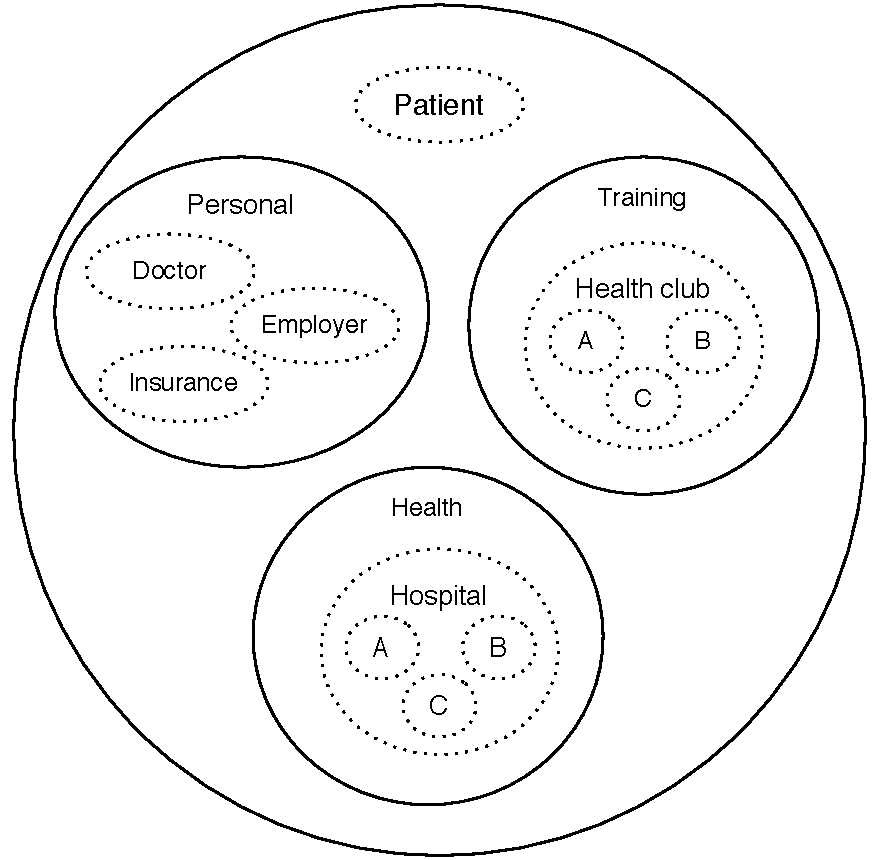
\includegraphics[width=0.6\columnwidth]{figures/mapping.pdf}
	     	\caption{Attributes are drawn with dashed borders. Categories with solid borders.}
			\label{fig:mapping}
		\end{figure}
	
	\subsection{Phases}
		The scheme has the following phases.
	
		\begin{description}
			\item[Setup]
			The client generates a master key and public key for each category.
			\item[Keygen]
			Based on the mappings, for each party for a given category, a secret key will be generated. To generate a secret key, the master key is used. Therefore, if the master key stays with the client, no other secret keys can be generated.
			\item[Encrypt]
			Given a message, category and receiving parties, the message will be encrypted with the public key for the given category with the policy based on the parties. The category is added as plain metadata to the ciphertext.
			\item[Decrypt]
			For a given ciphertext, decide which secret key to use based on the associated meta data. Then, decrypt the ciphertext.
		\end{description}
		
		Section \ref{sec:architecture} will provide more details about unfolding the parties to attributes.
		
		In the rest of this document, we often refer to the public key as the write key and the secret key as the read key. This is due to the fact that the public key is send to a party to grant write access.
    
\section{Implementation}
	This section describes the practical implementation of the assignment.
	
	\subsection{Used libraries}
		All software is written in Python. To create web pages, the Django Framework\footnote{\url{https://www.djangoproject.com/}} is used. The CP-ABE encryption is provided by the Charm Crypto\footnote{\url{http://www.charm-crypto.com/}} library by Akinyele, Green and Ruben \cite{cryptoeprint:2011:617}. AES encryption is provided by the Python Cryptographic Toolkit\footnote{\url{https://www.dlitz.net/software/pycrypto/}}. Web pages are rendered with the help of Bootstrap\footnote{\url{http://getbootstrap.com/}}, a front-end framework.
	
	\subsection{Architecture}\label{sec:architecture}
		The implementation consist of two parts. The first part is a storage server which does nothing more than saving records and providing records. The client part is a web application for all parties, but in a real situation, we assume that each type of party would have access to a own terminal to access PHR's. In fact, if it would be possible to have the server provide a GUI if we could implement CP-ABE in pure JavaScript (so encryption can stay local). Figure \ref{fig:architecture} depicts this architecture.
		
		\begin{figure}[H]
	        \centering
            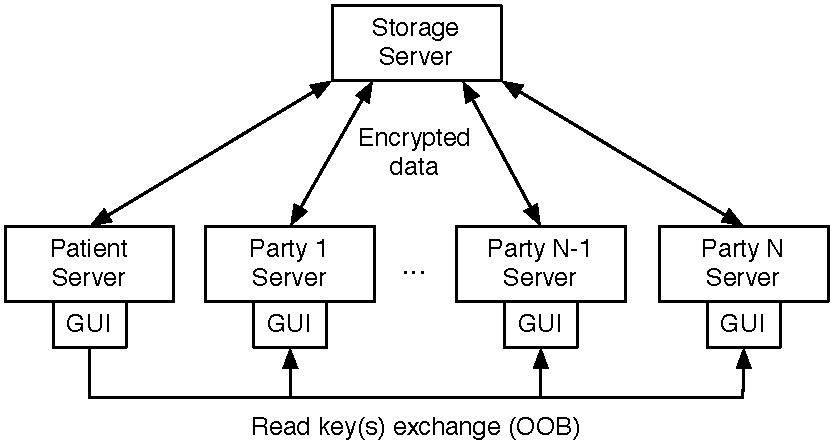
\includegraphics[width=0.75\columnwidth]{figures/architecture.pdf}
	     	\caption{Overview of architecture where the patient and several parties exchange data.}
			\label{fig:architecture}
		\end{figure}
	
		When a patient wants to create a PHR, he queries the server for the public system parameters. The system parameters include the categories, the involved parties and the mappings. The mappings describe for which party the client will generate read key with what attributes. For example, a mapping from \texttt{PERSONAL => EMPLOYER, INSURANCE, HOSPITAL+A+B} will result in read keys based on the master key for the category personal data. Employer will receive the attribute \texttt{EMPLOYER} and the Insurance the attribute \texttt{INSURANCE}. Hospital-A and Hospital-B will both get their own attribute \texttt{A} and \texttt{B}, but also the shared attribute \texttt{HOSPITAL}. Keys should be distributed in a secure way, preferably out-of-band (OOB).
		
		Encryption is done by specifying the plaintext, the category and the parties. The actual plaintext is encrypted with AES in CBC mode. The key for AES is the hash of a random element of the group where the CP-ABE scheme operates on. This random element is encrypted with the attributes for the receiver and added to the AES ciphertext, so the decrypting party can resolve the AES key. To generate a policy for the CP-ABE scheme, the given list of parties is unfolded. We use Python tuples and lists to define which parties have access and convert those to policy strings. Some examples (Python to policies):
		
		\begin{itemize}
			\item \texttt{[DOCTOR]} $\rightarrow$ \texttt{DOCTOR}
			\item \texttt{[HOSPITAL-A]} $\rightarrow$ \texttt{(HOSPITAL and A)}
			\item \texttt{[INSURANCE, DOCTOR]} $\rightarrow$ \texttt{INSURANCE or DOCTOR}
			\item \texttt{(INSURANCE, DOCTOR)} $\rightarrow$ \texttt{INSURANCE and DOCTOR}
			\item \texttt{[HOSPITAL, DOCTOR]} $\rightarrow$ \texttt{((HOSPITAL and A) or (HOSPITAL and B) or (HOSPITAL and C)) or DOCTOR}
			\item \texttt{[(HOSPITAL-A, HOSPITAL-B), INSURANCE]} $\rightarrow$ \texttt{((HOSPITAL and A) and (HOSPITAL and B)) or INSURANCE}
		\end{itemize}
		
		Above conversions allow us to build policies much more dynamic and coupled with our protocol. Our implementation validates all categories and parties specified during encryption. This means one cannot specify parties or categories that are not part of the system. A ciphertext contains a little bit of meta data that can be read without decrypting. This way, a receiving party knows to which category the ciphertext belongs and thus which read key(s) to consider.
		
		Sharing a write key is similar to encrypting data. There is only one write key per category and this key is generated during the creation of a PHR. The patient grants another party write access by encrypting the write key with the read key of the party or parties and uploads it to the server. Then, the party who will receive a key, retrieves this key from the server and decrypts it. The write key is added to the key chain. Now, the party can encrypt data.
		
		In short, one can consider our implementation as a strict extension layer between the actual CP-ABE scheme and the user.
				
		All business logic is documented and tested. We refer to the source code and README for an in-depth overview.
	
	\subsection{Database model}
		The role of the database is minimal. This resulted in a very small database model. The model is flexible, so we are not limited to any number of categories or parties.
		
		\textbf{Record}
		\begin{itemize}
			\item \textbf{ID} - The record ID.
			\item \textbf{Name} - Name of the record. Besides identification, not used for other purposes.
		\end{itemize}
		
		\textbf{Record item}
		\begin{itemize}
			\item \textbf{ID} - The record item ID.
			\item \textbf{Record ID} - The ID of the record this record item belongs to.
			\item \textbf{Category} - Text representation of the category this record item belongs to.
			\item \textbf{ciphertext} - Actual ciphertext.
		\end{itemize}
		
		\textbf{Key}
		\begin{itemize}
			\item \textbf{ID} - The record item ID.
			\item \textbf{Record ID} - The ID of the record this key belongs to.
			\item \textbf{Category} - Text representation of the category this key belongs to.
			\item \textbf{Key ciphertext} - Actual ciphertext containing the key.
		\end{itemize}
	
		ciphertext is saved in a Base64 encoded string.
	
	\subsection{Verification of requirements}
		The assignment considers the following requirements:
		
		\begin{enumerate}
			\item{A patient can insert personal health data into his \textit{own} record.}
			\item{A patient can provide his doctor, his insurance, and his employer with read access to (parts of) his health record.}
			\item{A hospital can insert patient health data for any patient that has been treated by \textit{that} hospital.}
			\item{A health club can insert training-related health data to any patient record that is a member of \textit{that} club.}
		\end{enumerate}
		
		To show that our system fulfills the requirements, we show a few use cases operated via the command line interface. One can play all use cases and should see similar results.
		
		\subsubsection{Creating a PHR}\label{sec:usecase_1}
			Since the patient is in control of his own PHR, he is responsible for creating one.
		
			\begin{lstlisting}
>>> python manage.py phr_create patient.json http://127.0.0.1:8000 "Patient record"
BEGIN SECRET READ FOR KEYS DOCTOR
(...truncated for clearance...)
END SECRET READ KEYS FOR DOCTOR

BEGIN SECRET READ FOR KEYS HOSPITAL-A
(...truncated for clearance...)
END SECRET READ KEYS FOR HOSPITAL-A

...

BEGIN SECRET READ FOR KEYS EMPLOYER
(...truncated for clearance...)
END SECRET READ KEYS FOR EMPLOYER

BEGIN SECRET READ FOR KEYS INSURANCE
(...truncated for clearance...)
END SECRET READ KEYS FOR INSURANCE
			\end{lstlisting}
		
			After running this command, all the secret reading keys for all the parties are generated. Each key has a bit of meta data encoded to connect to the right PHR. The mapping (see section \ref{sec:mappings}) defines who will get initial read access to which category of data. The patient should take care of distributing the keys, preferably via an out-of-band channel.
		
			A patient can encrypt data for other parties even if the keys have not yet been distributed.
		
		\subsubsection{Writing data}\label{sec:usecase_2}
			The patient decides to encrypt two messages. The first message can be read by his doctor, the second one by his insurance and his employer. They have access to the personal category of data.
		
			\begin{lstlisting}
>>> python manage.py phr_encrypt patient.json PERSONAL DOCTOR "Hi, Doctor!"
Uploaded to record item ID 55
>>> python manage.py phr_encrypt patient.json PERSONAL INSURANCE,EMPLOYER "Hi, Insurance and Employer!"
Uploaded to record item ID 56
			\end{lstlisting}
		
			The identifiers correspond to the items in the PHR of the patient. To verify that the patient has read access, he will decrypt the data he sent to the server.
		
			\begin{lstlisting}
>>> python manage.py phr_decrypt patient.json 55
Record item content:

Hi, Doctor
>>> python manage.py phr_decrypt patient.json 56
Record item content:

Hi, Insurance and Employer
			\end{lstlisting}
		
		\subsubsection{Granting write access}\label{sec:usecase_3}
			By default, no other party has write access. The patient should grant write access for all parties or sub parties.
		
			Let's assume the patient wants to grant Hospital-A write access.
			
			\begin{lstlisting}		
>>> python manage.py phr_grant patient.json HEALTH HOSPITAL-A
Granted key for category HEALTH with key ID 22
			\end{lstlisting}
			
			The write key is encrypted for party Hospital-A. If the patient wanted, he could give all hospitals write access by specifying the Hospital party instead of Hospital-A.
		
		\subsubsection{Connecting to a PHR}\label{sec:usecase_4}
			In this step, the keys have been safely distributed to each party. We let each party connect to the PHR of the client.
		
			\begin{lstlisting}
>>> python manage.py phr_connect doctor.json http://127.0.0.1:8000
Paste the keys data, excluding the BEGIN and END block: (...paste key for doctor...)
Connected to record ID 28

...

>>> python manage.py phr_connect insurance.json http://127.0.0.1:8000
Paste the keys data, excluding the BEGIN and END block: (...paste key insurance...)
Connected to record ID 28
			\end{lstlisting}
			
		\subsubsection{Reading data}\label{sec:usecase_5}
			In the first step, we encrypted two messages. One for only the doctor (\#55), and one for both the insurance and employer (\#56). 
			
			First the doctor:
			
			\begin{lstlisting}
>>> python manage.py phr_decrypt doctor.json 55
Record item content:

Hi, Doctor
>>> python manage.py phr_decrypt doctor.json 56
Cannot decrypt record item
			\end{lstlisting}

			Then the employer and insurance:

			\begin{lstlisting}
>>> python manage.py phr_decrypt employer.json 56
Record item content:

Hi, Insurance and Employer
>>> python manage.py phr_decrypt insurance.json 56
Record item content:

Hi, Insurance and Employer
>>> python manage.py phr_decrypt employer.json 55
Cannot decrypt record item
>>> python manage.py phr_decrypt insurance.json 55
Cannot decrypt record item
			\end{lstlisting}
			
			And to be sure, we verify the health club and hospital cannot read the messages (they have read access to different categories).

			\begin{lstlisting}
>>> python manage.py phr_decrypt healthclub-a.json 55
Cannot decrypt record item
>>> python manage.py phr_decrypt healthclub-a.json 56
Cannot decrypt record item
>>> python manage.py phr_decrypt hospital-a.json 55
Cannot decrypt record item
>>> python manage.py phr_decrypt hospital-a.json 56
Cannot decrypt record item
			\end{lstlisting}
		
		\subsubsection{Retrieving write access}\label{sec:usecase_6}
			In use case \ref{sec:usecase_3} we provided Hospital-A with a write key. The party should retrieve the key from the server.
			
			\begin{lstlisting}
>>> python manage.py phr_retrieve hospital-a.json HEALTH
Key(s) imported for HEALTH.
			\end{lstlisting}
			
			The same does not work for other parties, e.g. Hospital-B and Health Club-A:
		
			\begin{lstlisting}
>>> python manage.py phr_retrieve hospital-b.json HEALTH
No new key(s) imported.
>>> python manage.py phr_retrieve healtclub-a.json HEALTH
No new key(s) imported.
			\end{lstlisting}
		
			Just to verify the keys are imported, one can issue the status command.
			
			\begin{lstlisting}
>>> python manage.py phr_status hospital-a.json
Host:        http://127.0.0.1:8000
Categories:  PERSONAL, HEALTH, TRAINING
Parties:     DOCTOR, INSURANCE, EMPLOYER, HOSPITAL+A+B+C, HEALTHCLUB+A+B+C
Mappings:    PERSONAL -> DOCTOR, INSURANCE, EMPLOYER
             TRAINING -> HEALTHCLUB
             HEALTH -> HOSPITAL

Record ID:   28
Record name: Patient record
Record role: HOSPITAL-A

Master keys: <not set>
Public keys: HEALTH
Secret keys: HOSPITAL-A -> HEALTH
			\end{lstlisting}
			
			For the above case, Hospital-A has connected to the right record, is able to decrypt messages for Hospital-A in the Health category and can encrypt messages for the Health category. Note that the master keys are not available, so Hospital-A cannot generate new keys (only the patient can do this).
		
		\subsubsection{Writing a reply}\label{sec:usecase_7}
			Now Hospital-A has write access, he can write data to the Health category. To verify this, we will write a message to the Health category only for the patient and one to all hospitals.
			
			\begin{lstlisting}
>>> python manage.py phr_encrypt hospital-a.json HEALTH HOSPITAL "Hello patient!""
Uploaded to record item ID 57
>>> python manage.py phr_encrypt hospital-a.json HEALTH HOSPITAL "Hello patient and other hospitals!""
Uploaded to record item ID 58
			\end{lstlisting}
			
			To conclude, each addressed party will decode it:

			\begin{lstlisting}
>>> python manage.py phr_decrypt hospital-a.json 57
Record item content:

Hello patient!
>>> python manage.py phr_decrypt hospital-b.json 57
Cannot decrypt record item
>>> python manage.py phr_decrypt hospital-c.json 57
Cannot decrypt record item
>>> python manage.py phr_decrypt hospital-a.json 58
Record item content:

Hello patient and other hospitals!
>>> python manage.py phr_decrypt hospital-b.json 58
Record item content:

Hello patient and other hospitals!

>>> python manage.py phr_decrypt hospital-c.json 58
Record item content:

Hello patient and other hospitals!
			\end{lstlisting}

			And the patient:

			\begin{lstlisting}
>>> python manage.py phr_decrypt patient.json 57
Record item content:

Hello patient!
>>> python manage.py phr_decrypt patient.json 58
Record item content:

Hello patient and other hospitals!
			\end{lstlisting}
		
		\subsubsection{A second patient record}\label{sec:usecase_8}
			A patient is in control of his own PHR and has all the keys to read and write. In this use case, we show that another patient cannot decrypt a record item that does not belong to him. Because the API requires the user to specify a record item ID and the record ID in order to communicate with the server, we modified it for this use case to only require the record item ID. Without this modification, patient two would not be able to query for record items that are not part of his PHR.
			
			First, we create a second patient.
			
			\begin{lstlisting}
>>> python manage.py phr_create patient.json http://127.0.0.1:8000 "Patient two record"
BEGIN SECRET READ FOR KEYS DOCTOR
(...truncated for clearance...)
END SECRET READ KEYS FOR DOCTOR

BEGIN SECRET READ FOR KEYS HOSPITAL-A
(...truncated for clearance...)
END SECRET READ KEYS FOR HOSPITAL-A

...

BEGIN SECRET READ FOR KEYS EMPLOYER
(...truncated for clearance...)
END SECRET READ KEYS FOR EMPLOYER

BEGIN SECRET READ FOR KEYS INSURANCE
(...truncated for clearance...)
END SECRET READ KEYS FOR INSURANCE
			\end{lstlisting}
			
			Then, we connect the (same) doctor to that record, since patient one encrypted a message (\#55) for him.
			
			\begin{lstlisting}
>>> python manage.py phr_connect doctor-patient-two.json http://127.0.0.1:8000
Paste the keys data, excluding the BEGIN and END block: (...paste key for doctor...)
Connected to record ID 29
			\end{lstlisting}
			
			It should be sufficient to show that both the patient two and the doctor with the other data file cannot read message from patient one.
			
			\begin{lstlisting}
>>> python manage.py phr_decrypt patient-two.json 55
Cannot decrypt record item
>>> python manage.py phr_decrypt doctor-patient-two.json 55
Cannot decrypt record item
			\end{lstlisting}
			
		\subsubsection{Undecryptable data}\label{sec:usecase_9}
			It is possible to encrypt data for a category with a write key for a party not in the mapping. Consider Hospital-A encrypting for Health Club-A, while Health Club-A has no access to the category Health.
			
			\begin{lstlisting}
>>> python manage.py phr_encrypt hospital-a HEALTH HEALTCLUB-A "Undecryptable, for now..."
Uploaded to record item ID 59
>>> python manage.py phr_decrypt patient.json 59
Cannot decrypt record item
			\end{lstlisting}
			
			As can be seen, even the patient cannot decrypt it anymore, and if the patient cannot read it, no other party can read it. However, the patient could decide to generate a read key for it.
		
		\subsubsection{Conclusion}
			We conclude this section with a table representing which requirement is fulfilled by which use case.

			\begin{table}[h!]
				\center
			    \begin{tabular}{| l | l | l | l | l |} \hline
			    ~                            & Requirement 1 & Requirement 2 & Requirement 3 & Requirement 4 \\ \hline
			    Use case \ref{sec:usecase_1} & ~             & X             & ~             & ~             \\ \hline
			    Use case \ref{sec:usecase_2} & X             & ~             & ~             & ~             \\ \hline
			    Use case \ref{sec:usecase_3} & ~             & ~             & X             & X             \\ \hline
			    Use case \ref{sec:usecase_4} & ~             & X             & ~             & ~             \\ \hline
			    Use case \ref{sec:usecase_5} & ~             & X             & ~             & ~             \\ \hline
			    Use case \ref{sec:usecase_6} & ~             & ~             & X             & X             \\ \hline
			    Use case \ref{sec:usecase_7} & ~             & ~             & X             & X             \\ \hline
			    Use case \ref{sec:usecase_8} & X             & ~             & ~             & ~             \\ \hline
			    Use case \ref{sec:usecase_9} & X             & ~             & ~             & ~             \\ \hline
			    \end{tabular}
			
				\caption{Overview of which use cases cover which requirements.}
			\end{table}
	
\section{Discussion}

	\subsection{Authentication}
		Our implementation does not authenticate a party to the server and visa versa. This does not have any impact on the secrecy of the data, since only the parties with the correct keys, distributed via secure channels, can read or write data. The server cannot learn anything from the data. However, since anyone can upload data to our server, a lot of false and corrupt data may be stored in the database. A client cannot delete data, since the server does not know the client. The same holds for keys uploaded to the server. Once data is sent, you should consider the ciphertext compromised.
		
		Since authentication is out of the scope of this assignment, we have not implemented a counter measure.
		
	\subsection{Number of keys}
		There are a lot of keys to be generated during the setup and keygen phase. There are $N$ master keys and $N$ public keys for $N$ categories. Based on the mapping, each party having read access gets at least one read key. If the number of parties (and sub parties) grow, the number of read keys grows too.
		
		Only the patient has to store all the keys. The key size in the chosen CP-ABE scheme is lineair with the number of attributes. All other parties should only store their read and write keys.
	
	\subsection{Key sharing}
		For each category of data, there is only one master key and one write key. The write key is shared among the parties if they want write access. If a party is malicious, he could impersonate another party or spread the write key. Keys cannot be revoked, unless the patient generates new keys.
		
		In the given assignment this is not a problem. First of all, we assume honest parties. Second, only write access is granted to the hospital and health club, both operating on a different category of data. If one would abuse a key, it would be very easy to trace it back to the malicious party.

\section{References}
	\bibliography{references}
	\bibliographystyle{plain}

\end{document}